
  
\documentclass{exam}
\usepackage[utf8]{inputenc}
\usepackage{upgreek}
\usepackage[margin=1in]{geometry}
\usepackage{amsmath,amssymb}
\usepackage{multicol}
\usepackage{stmaryrd}
\usepackage{graphicx}
\usepackage{caption}
\usepackage{tikz}
\usepackage{dsfont}
\usepackage{enumitem}
\usepackage{hyperref}
\usetikzlibrary{matrix}
\newcommand\tab[1][1cm]{\hspace*{#1}}
\pagestyle{head}
\firstpageheader{}{}{}
\runningheader{\examnum}{\class}{\name}
\runningheadrule
\newcommand{\class}{Fundamentos de bases de datos}
\newcommand{\term}{Facultad de Ciencias UNAM}
\newcommand{\examnum}{Practica 01 - Bitácora}
\newcommand{\examdate}{07/03/2022}
\newcommand{\name}{Yamil Salazar Gonzalez - 306037445}
\begin{document}

\noindent
\begin{tabular*}{\textwidth}{l @{\extracolsep{\fill}} r @{\extracolsep{6pt}} l}
\textbf{\class} & \textbf{\term}\\
\textbf{\examnum} & \textbf{\name}\\
\textbf{\examdate}
\end{tabular*}\\
\rule[2ex]{\textwidth}{2pt}

\section*{Bitácora}

\subsection*{Sistema operativo y versión}

	\begin{itemize}
		\item Procesador: AMD Ryzen 5 345U with Radeon VEga Mobile Gfx 2.10GHz
		\item RAM 8.00 GB
		\item Sistema operativo de 64 bits, procesador basado en x64 (Windows 11)
		\item Fabricante: Dell
	\end{itemize}

\subsection*{Versión de la instalación}
	Windows 11 Home Single Language versión 21H2; Versión del SO 22000.493


\subsection*{Tiempo requerido}

El tiempo requerido fue de aproximadamente 40 min

\subsection*{Explicación del paso a paso}

    \begin{enumerate}
        \item Entre a la página y descargue la versión para Windows
        \begin{figure}[h]
            \centering
            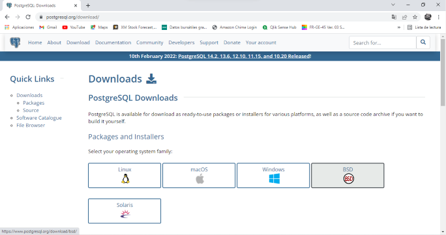
\includegraphics{imgSalazar/I_01.png}
        \end{figure}
        \begin{figure}[h]
            \centering
            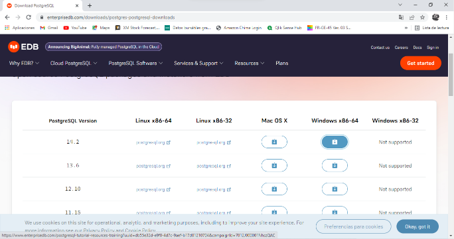
\includegraphics{imgSalazar/I_02.png}
        \end{figure}
        \newpage
        \item Seguí las instrucciones del instalador
        \begin{figure}[h]
            \centering
            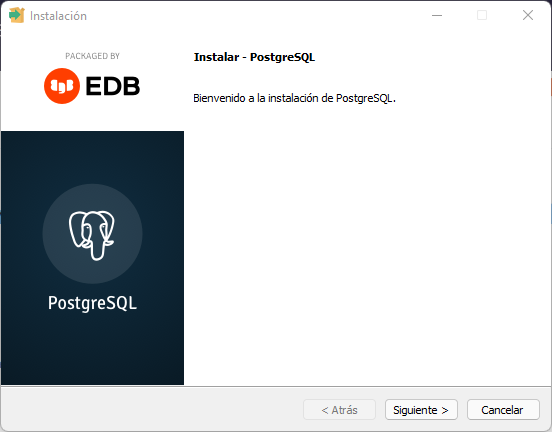
\includegraphics[width = 10 cm]{imgSalazar/I_03.png}
        \end{figure}
        \newpage
        \item seleccione la carpeta en donde se instalo
        \begin{figure}[h]
            \centering
            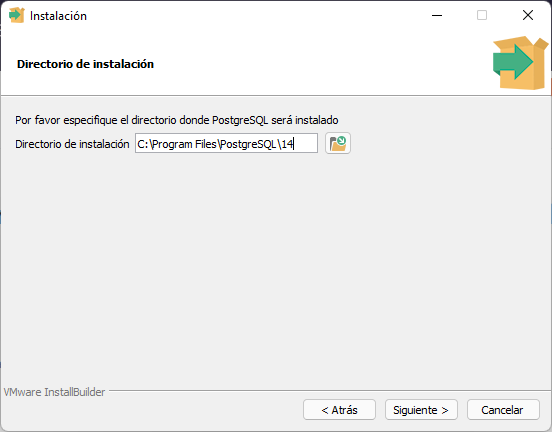
\includegraphics[width = 10 cm]{imgSalazar/I_04.png}
        \end{figure}
        \item La selección de componentes a instalar
        \begin{figure}[h]
            \centering
            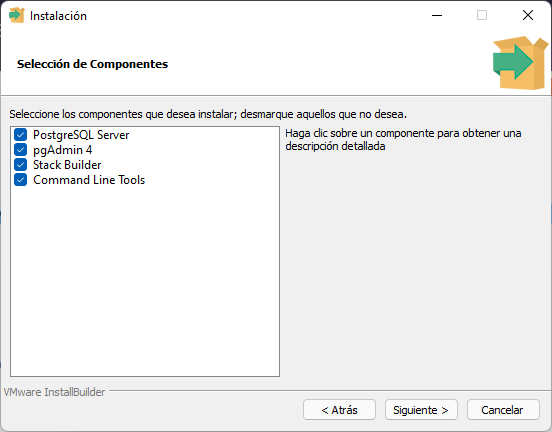
\includegraphics[width = 10 cm]{imgSalazar/I_05.png}
        \end{figure}
        \newpage
        \item En donde se almacenarán los datos
        \begin{figure}[h]
            \centering
            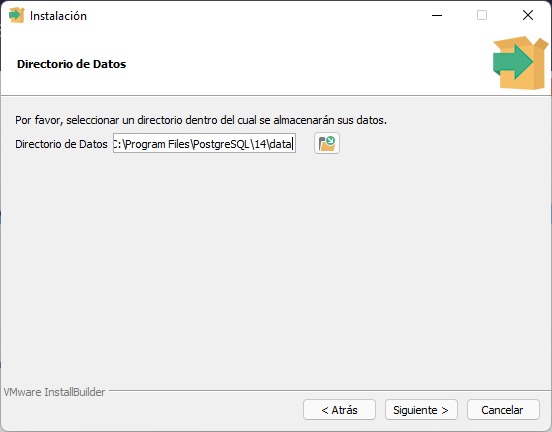
\includegraphics[width = 10 cm]{imgSalazar/I_06.png}
        \end{figure}
        \item Creación de la contraseña para el superusuario
        \begin{figure}[h]
            \centering
            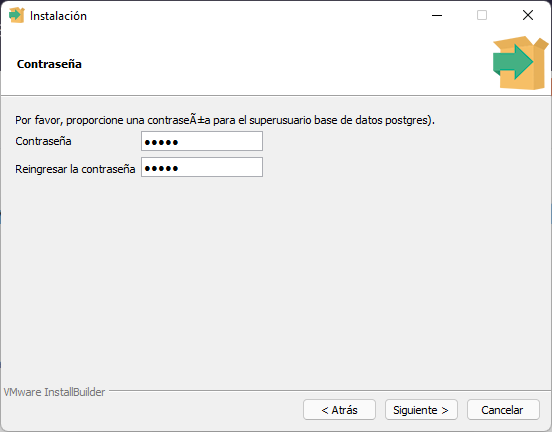
\includegraphics[width = 10 cm]{imgSalazar/I_07.png}
        \end{figure}
        \newpage
        \item Selección del puerto que se usará
        \begin{figure}[h]
            \centering
            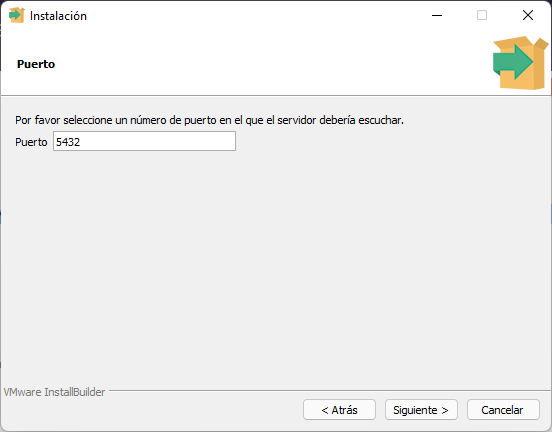
\includegraphics[width = 10 cm]{imgSalazar/I_08.png}
        \end{figure}
        \item La configuración del cluster
        \begin{figure}[h]
            \centering
            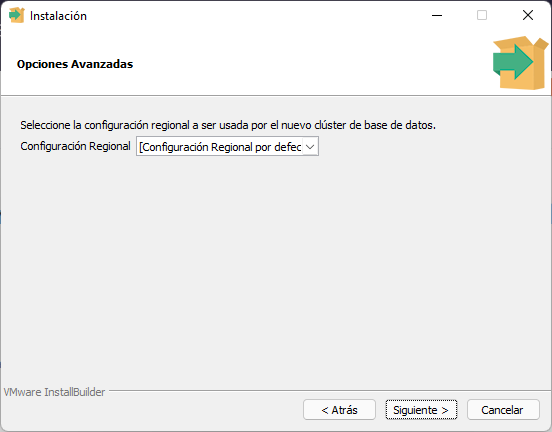
\includegraphics[width = 10 cm]{imgSalazar/I_09.png}
        \end{figure}
        \newpage
        \item Instalando
        \begin{figure}[h]
            \centering
            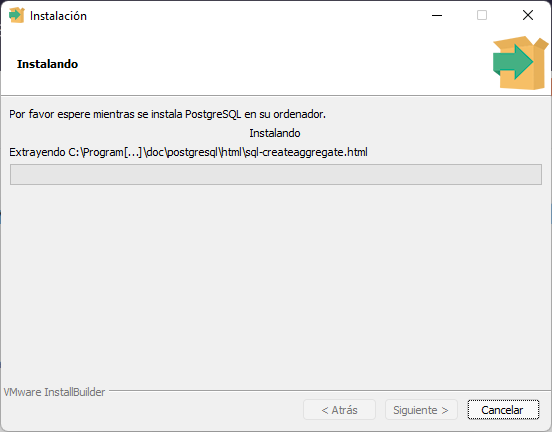
\includegraphics[width = 10 cm]{imgSalazar/I_10.png}
        \end{figure}
        \item Fin de la instalación
        \begin{figure}[h]
            \centering
            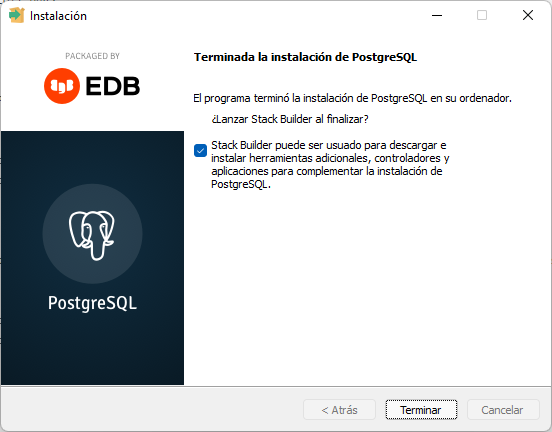
\includegraphics[width = 10 cm]{imgSalazar/I_11.png}
        \end{figure}
        
    \end{enumerate}

\subsection*{Comentarios y problemas}

Al poder usar el instalador de Windows para realizar esta instalación, no tuve problemas para hacerlo.


\end{document}